\chapter{Test Equation}
This course is about scientific methods for solving differential equation of various types. As such, much of our focus will be on different methods to do so. We will discuss the strengths and limitations of these methods. For the most of the report we will deal with initial value problems (IVP) that can be written on the form
\begin{align}
    \dot{x}(t) &= f(t,x(t),p), & x(t_0) = x_0,
\end{align}
where $x \in \probR ^{n_x}$ and $p \in \probR ^{n_p}$. 

We will discuss several characteristics for the various scientific methods, however, one of the more important is how they converge. In order to compare characteristics of convergence between methods, we need to agree on some standard way of testing. In this regard we introduce the \textit{test equation}. The test equation is defined by the IVP 
\begin{align}
    \dot{x}(t) &= \lambda \cdot x(t), & x(t_0)=x_0, \ \lambda=c,
\end{align}
with $\lambda \in \mathcal{C}$.
Notice that the test equation gives rise to a relatively simple problem. Form the study of dynamical systems we immediately recognize that the test equation will be asymptotic stable for $Re(\lambda)<0$, it will be stable for $Re(\lambda) \leq 0$ and unstable for $Re(\lambda)>0$ cf. Perko\cite{Perko}. 

\section{Analytical solution to test equation}
Let consider a concrete example of the test equation, namely 
\begin{align}
    \dot{x}(t) &= -x(t), & x(t_0)=1. \label{eq:ivp1}
\end{align}
Notice that $\lambda=-1$, so we know the test equation is asymptotically stable in this example. Furthermore, the analytic solution is cf. Perko\cite{Perko} found by
\begin{align}
    x(t) &= \exp \left [ \lambda \cdot t  \right ] \cdot x_0 \quad \Rightarrow \\
    x(t) &=  \exp \left [ - t  \right ].
\end{align}
It is evident that the analytic solution goes to $0$ for $t \rightarrow \infty$, so it \textit{is} in fact asymptotically stable as expected. 


\section{Local and global truncation errors}
Besides how the scientific methods converge another important aspect is their errors. Since all methods are numerical methods there will be some difference between the analytical solution---if such exists---and the numerically obtained one. We divide these differences into two categories: \textit{Local truncation errors} and \textit{global truncation errors}. 

Let $0 \leq t$ denote some time, and let $h$ denote the step size of a numerical method. Further, let $\hat{x}(t)$ denote the solution to an IVP at time, $t$, by means of the numerical method. Let $z$ denote the analytical solution to the same IVP at $t+h$ starting at $\hat{x}(t)$. The local truncation error is then given by
\begin{align}
    \hat{e}_{t+h} = z - \hat{x}(t+h).
\end{align}
In layman terms, the local truncation error is the \textit{new} errors introduced at each step. 

Now let $x(t)$ denote the exact solution at time, t, starting at $x(t) = x_0$. The global truncation error is then given by
\begin{align}
    e_t = x(t)-\hat{x}(t).
\end{align}

Figure \ref{fig1:local_err0} display both the exact solution and a numerical solution to the IVP from Equation \ref{eq:ivp1}. Notice that the red lines indicate the local truncation error for each time step. The global truncation errors can at all times be found as the difference between the exact and the numeric solution.
\begin{figure}[H]
    \centering
    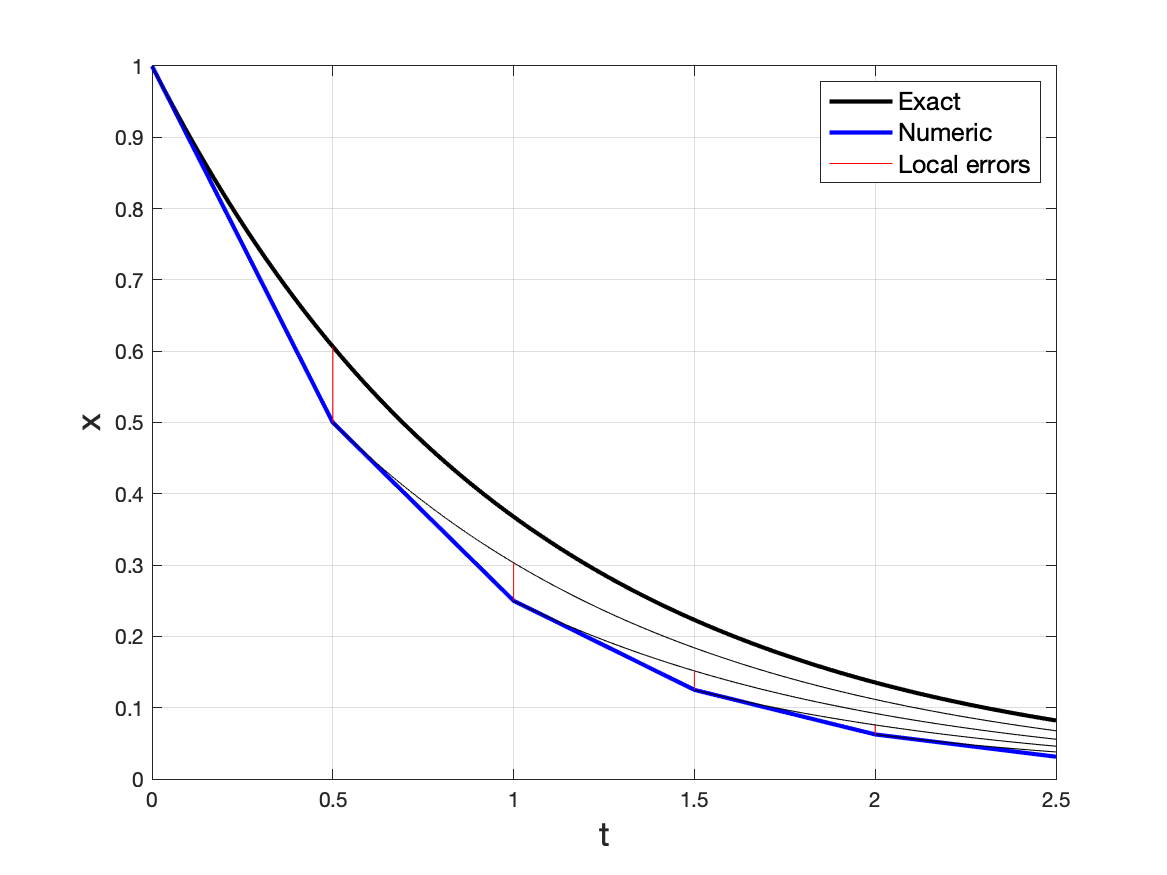
\includegraphics[width=10cm]{graphics/opg1/local_err0.png}
    \caption{Test equation with $\lambda=-1$ and $x_0=1$.}
    \label{fig1:local_err0}
\end{figure}


\section{Local and global truncation error on the test equation}
Obviously, both the local and global truncation errors depend on the method used---some methods will yield lower errors for the same step size, but might also be more demanding to compute. We will now compare a few different methods, namely 
\begin{itemize}
    \item[a)] the explicit Euler method (fixed step size),
    \item[b)] the implicit Euler method (fixed step size), and 
    \item[c)] the classical Runge-Kutta.
\end{itemize}
Specifically, we will use the methods in mention on the IVP from Equation \ref{eq:ivp1} with a fixed step size at $h=0.25$. Figure \ref{fig1:local_err1} shows the absolute value of the local truncation errors for the three methods. Notice that the errors are large initially but over time goes towards zero. This is because all three methods follow the behaviour of the exact solution to the test equation with these parameters---but more on that later. Also notice the difference between the explicit and implicit Euler methods and the classical Runge-Kutta (RK4). This difference is to do with the \textit{order} of the methods, which we will touch upon shortly.

\begin{figure}[H]
    \centering
    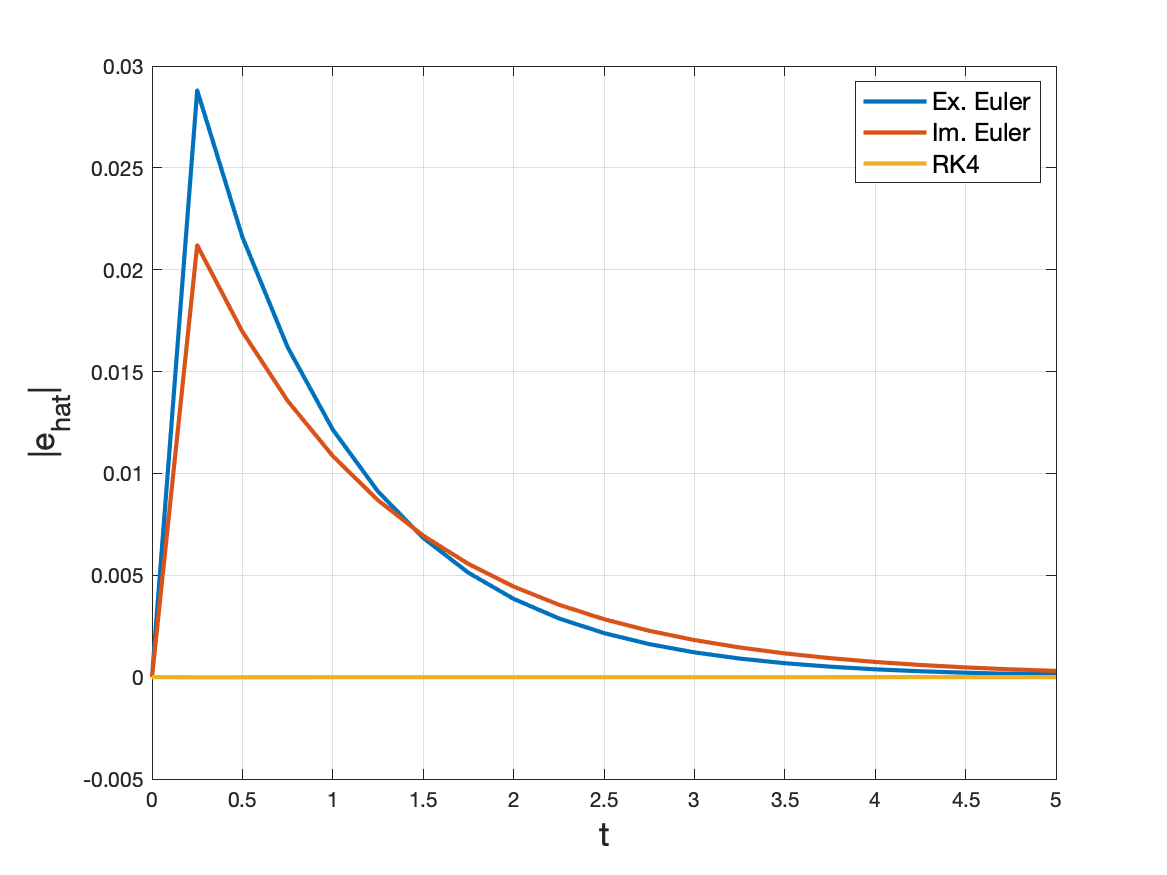
\includegraphics[width=10cm]{graphics/opg1/local_err1.png}
    \caption{Local truncation errors to test equation with $\lambda=-1$ and $x_0=1$ using different numerical methods.}
    \label{fig1:local_err1}
\end{figure}

Figure \ref{fig1:global_err1} shows the absolute value of the global truncation errors to the test equation with the given parameters for the three numerical methods in mention. Once again we see the behaviour where the errors are greatest initially and then decrease over time. This is again to do with the parameters in the test equation and the \textit{stability} of the methods used. Shortly, we will understand this better.

\begin{figure}[H]
    \centering
    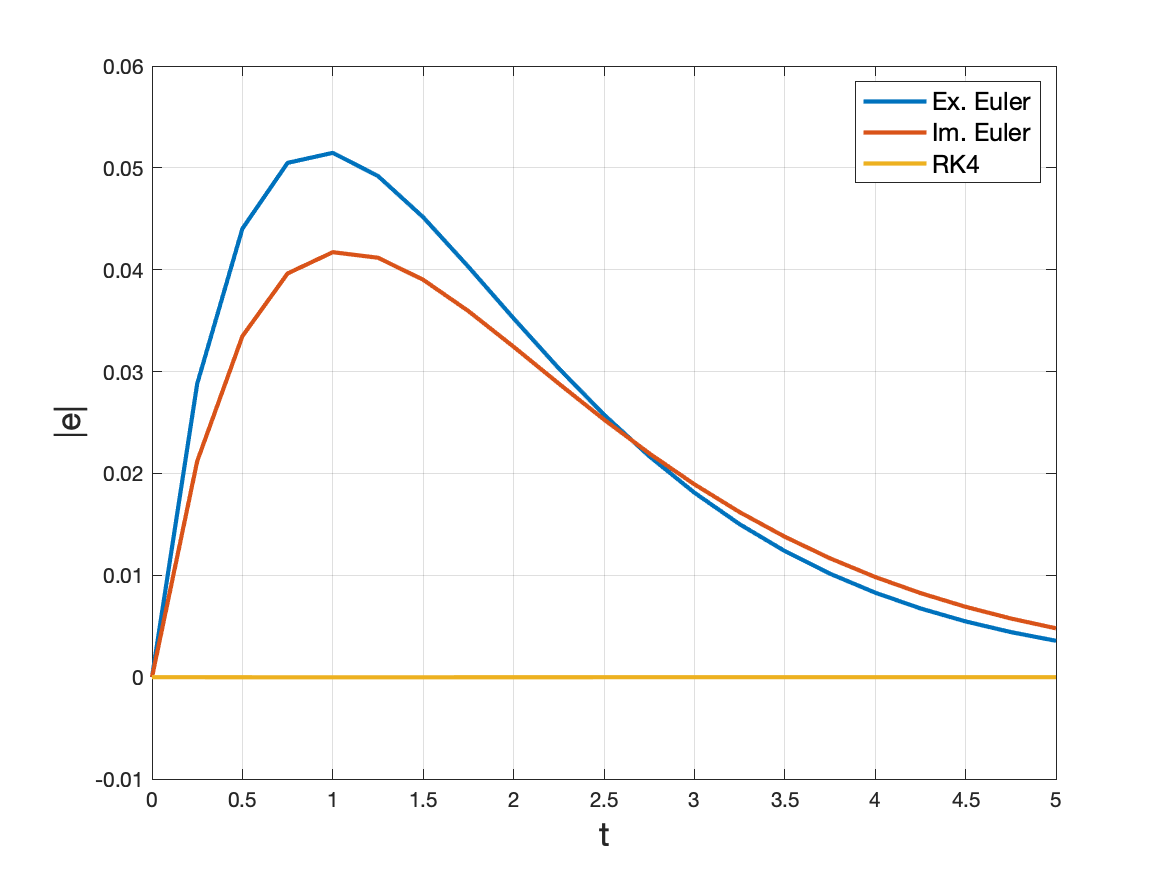
\includegraphics[width=10cm]{graphics/opg1/global_err1.png}
    \caption{Global truncation errors to test equation with $\lambda=-1$ and $x_0=1$ using different numerical methods.}
    \label{fig1:global_err1}
\end{figure}

\section{Local errors by step size}
The step size, $h$, plays an important role in the accuracy, i.e., the magnitude of local and/or global truncation errors, of any numerical method. Figure \ref{fig1:local_err2} shows the local error vs the time step for the numerical methods. Notice that the local truncation errors for both explicit and implicit Euler seem to roughly follow a linear trend. The local errors of the RK4 follow a higher order curve---from this plot alone it is difficult to determine the exact order.

\begin{figure}[H]
    \centering
    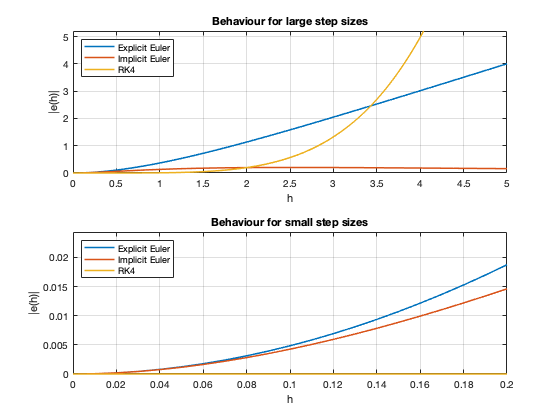
\includegraphics[width=10cm]{graphics/opg1/local_err_h.png}
    \caption{Local truncation errors as function of step size, $h$.}
    \label{fig1:local_err2}
\end{figure}

In fact, the local error has very much to do with the previously mentioned \textit{order} of the numerical method. Cf Ascher\cite{Ascher} a numerical method is said to have order $p$ if
\begin{align}
    e_t &= \mathcal{O}(h^p).
\end{align}
It turn out that the numerical methods in mention have order
\begin{align*}
    Explicit \ Euler:& \quad 1 \quad\quad\quad &&& \\
    Implicit \ Euler:& \quad 1 \quad\quad\quad &&& \\
    RK4:& \quad 4. \quad\quad\quad &&&
\end{align*}
The order of the methods will be shown later in this report.

\section{Global errors at t=1}
The order of the method has a large impact on the global truncation errors as just shown. However, the order also have a large impact on the global truncation errors. To demonstrate this, we re-use the IVP from Equation \ref{eq:ivp1}, at look at the global truncation error, i.e., the difference between the exact and the numerical solution, at $t=1$. We can do this for varying step sizes, $h$, and thereby get an idea of the impact. Figure \ref{fig1:err_t1} shows the absolute value of the global truncation errors at $t=1$, i.e., $|e_1|$. 

\begin{figure}[H]
    \centering
    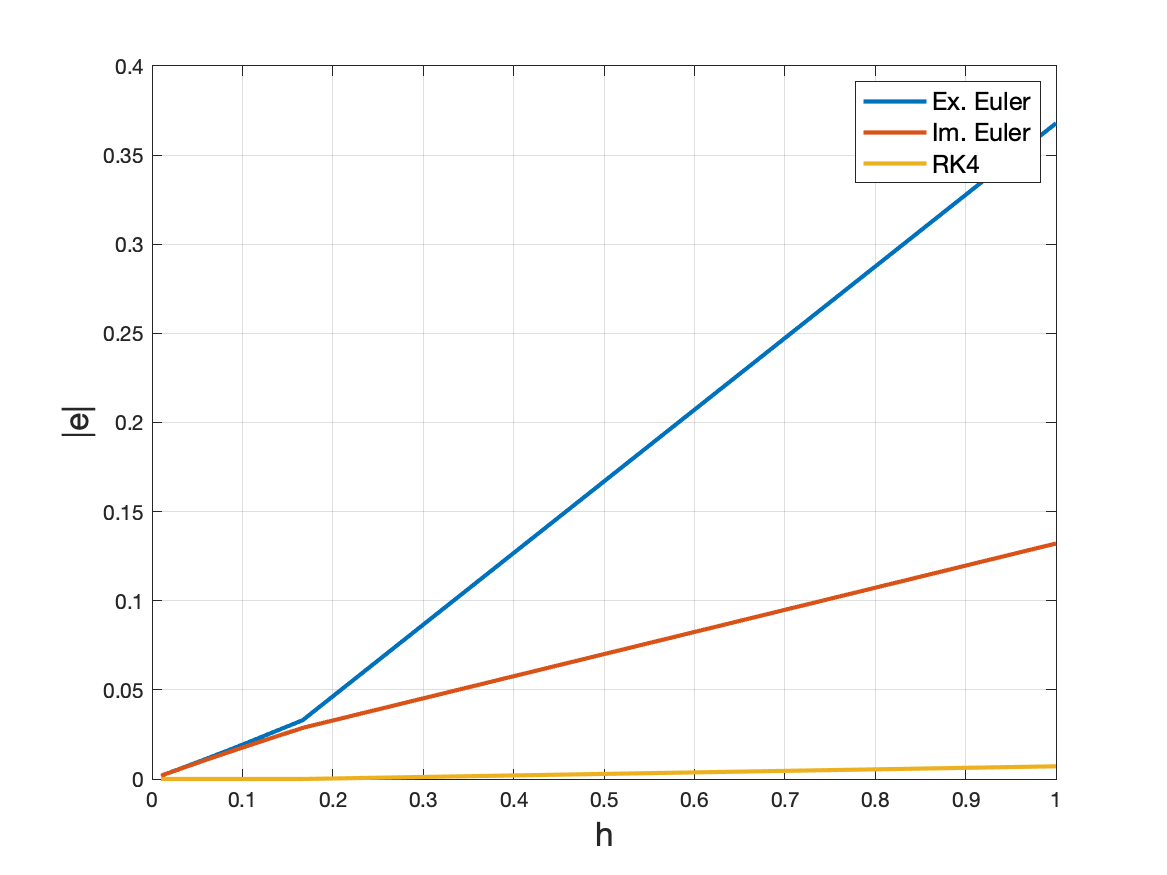
\includegraphics[width=10cm]{graphics/opg1/err_t1.png}
    \caption{Global truncation error to test equation with $\lambda=-1$ and $x_0=1$ using different numerical methods at $t=1$.}
    \label{fig1:err_t1}
\end{figure}

Notice that the absolute value of the global truncation errors of both the explicit and implicit Euler methods seem to increase linearly with the size of the time steps. This aligns with the order of the methods, since they are both methods of order 1. Since the classical Runge-Kutta method is of order 4, we would expect the global truncation error to follow $h^4$. However, based on this relatively small interval, it is difficult to see if that is actually the case. We can, however, see that the global truncation errors of RK4 are significantly lower than both the explicit and implicit Euler methods for the same time step sizes. 

\section{Stability of a numerical method}
As previously mentioned, \textit{stability}, i.e., how the methods converge, of numerical methods are an important characteristic of any numerical method. We have now introduced the test equation, and we will use this to say something about the stability of numerical methods. It is important to remember that stability is seen in this exact context, i.e., how the method perform on the test equation with a given set of parameters. 

Before we define exactly what we mean by stability of a numerical method, we need a little bit of framework. To investigate the properties of a numerical method, we write it on the form
\begin{align}
    x(t+h) &= R(\mu) x(t),
\end{align}
where the structure of $R(\cdot)$ depends on the numerical method used. 

A method is said to be \textit{stable} for some $\mu$ whenever $|R(\mu)| \leq 1$. Notice that \textit{stability} depends on the specific value for $\mu$. If we have that 
\begin{align}
    Re(\lambda) \leq 0 \quad \Leftrightarrow \quad |R(\mu)| \leq 1
\end{align}
we say that the method is \textit{A-stable}. Notice this means that for any $\lambda \leq 0$ we have stability, i.e., what we usually expect in the analytic case. 

If we further have that 
\begin{align}
    Re(\lambda) \rightarrow -\infty \quad \Rightarrow \quad |R(\mu)| \rightarrow 0
\end{align}
i.e., the method will converge in fewer steps when $\lambda$ becomes more negative, we say that the method is \textit{L-stable}. 

Let us look at a few examples. We will start with the explicit Euler method. The explicit Euler method is defined by 
\begin{align}
    x(t+h) &= x(t) + \lambda x(t) h \\
    &= (1+\lambda h) x(t).
\end{align}
So we have 
\begin{align}
    R(\mu) = 1 + \mu.
\end{align}
We can now define the stability region, $\mathcal{S}$, as the region where the method is stable. The stability region is therefore given by
\begin{align}
    \mathcal{S} = \left \{ \mu \in \mathcal{C} \ | \ |1+\mu| \leq 1 \right \}.
\end{align}

Figure \ref{fig1:ex_stability} shows stability region of the explicit Euler method. Notice that the method is only stable of a small circular region of $\mu=\lambda h$. Notice that this means that it is possible that the explicit Euler method does not converge, even if the exact solution does, i.e., the problem \textit{is} stable. It is therefore evident that the method is neither A nor L-stable.

\begin{figure}[H]
    \centering
    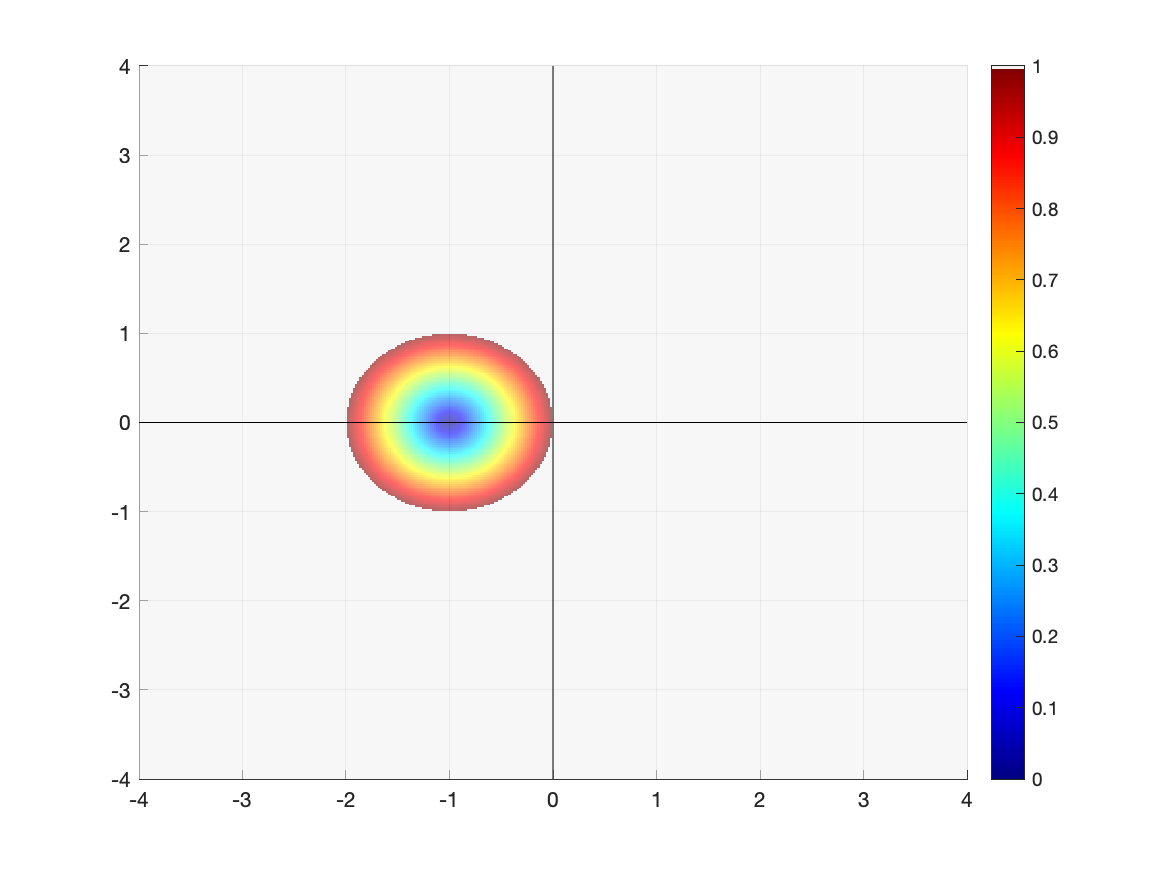
\includegraphics[width=10cm]{graphics/opg1/ex_stability.png}
    \caption{Stability region of the explicit Euler method on test equation. The colored region is the stable region.}
    \label{fig1:ex_stability}
\end{figure}


The implicit Euler method is given by
\begin{align}
    x(t+h) &= x(t) + \lambda x(t+h) h \\
    &= \frac{1}{1-\lambda h} x(t).
\end{align}
So we have 
\begin{align}
    R(\mu) = \frac{1}{1-\mu}.
\end{align}
We can now define the stability region, $\mathcal{S}$, for the implicit Euler method by
\begin{align}
    \mathcal{S} = \left \{ \mu \in \mathcal{C} \ | \ |\frac{1}{1-\mu}| \leq 1 \right \}.
\end{align}

Figure \ref{fig1:im_stability} shows the stability region of the implicit Euler method. Notice that a much larger area is stable than the for the explicit Euler method. In fact, the method is stable for all $Re(\lambda) \leq 0$, which tells us that the implicit Euler method is A-stable. Additionally, if we take a closer look at $R(\lambda h) = \frac{1}{1-\lambda h}$, we see that it goes towards $0$ for $\lambda \rightarrow -\infty$. Therefore the implicit Euler method is also L-stable. 

\begin{figure}[H]
    \centering
    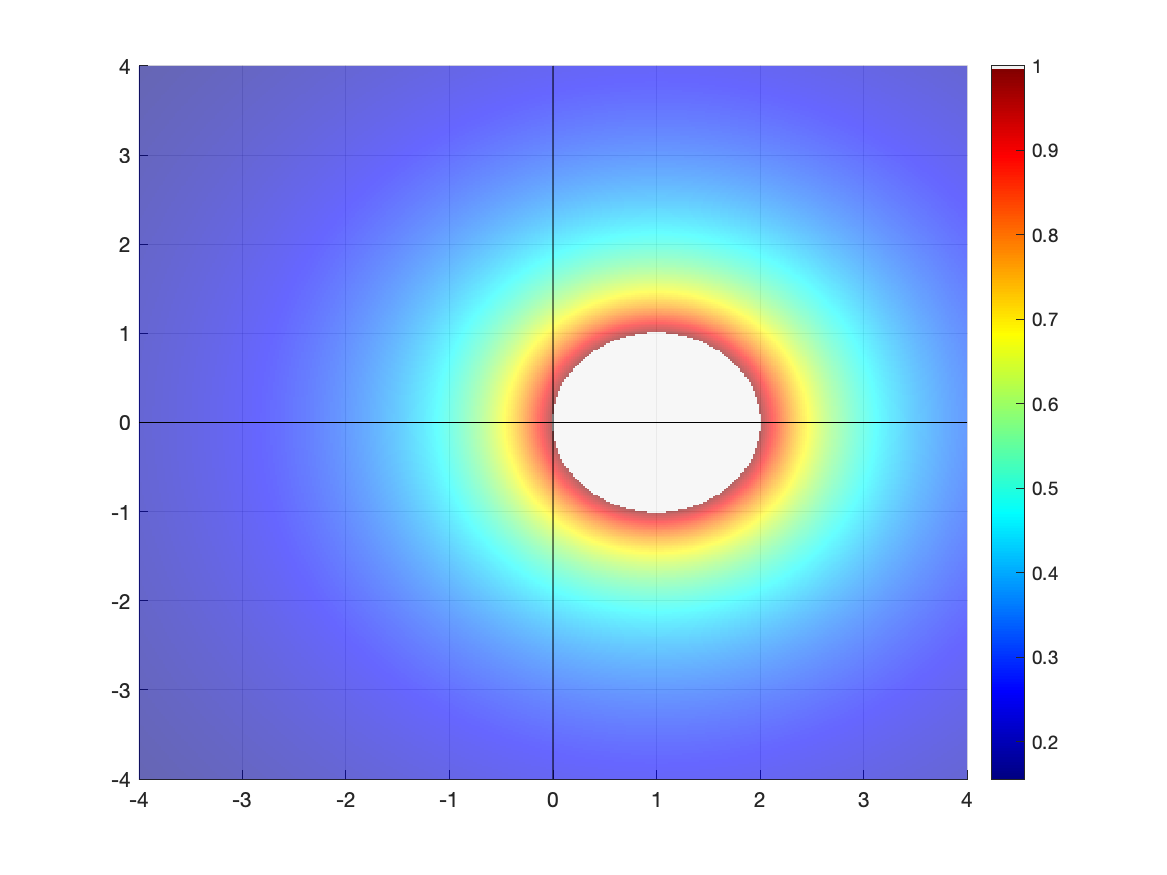
\includegraphics[width=10cm]{graphics/opg1/im_stability.png}
    \caption{Stability region of the implicit Euler method on test equation. The colored region is the stable region.}
    \label{fig1:im_stability}
\end{figure}

In fact, the implicit Euler method is \textit{too} stable. Notice that the method is stable even for some $Re(\lambda)>0$. This means that the implicit Euler method might converge even when the test equation is unstable! 

The classical Runge-Kutta method is a bit more complicated. We will therefore not derive the stability function, $R(\cdot)$ for RK4 here. Cf. Ascher\cite{Ascher}, the stability function for RK4 can be written as
\begin{align}
    R(\mu) = 1 + \mu + \frac{1}{2}\mu^2 + \frac{1}{6} \mu^3 + \frac{1}{24} \mu^4.
\end{align}
This gives us a region of stability, $\mathcal{S}$, as
\begin{align}
    \mathcal{S} = \left \{ \mu \in \mathcal{C} \ | \ | 1 + \mu + \frac{1}{2}\mu^2 + \frac{1}{6} \mu^3 + \frac{1}{24} \mu^4| \leq 1 \right \}.
\end{align}
Figure \ref{fig1:rk4_stability} shows the stability region for the classical Runge-Kutta method. Notice that the stability region is much like that of the explicit Euler method, in the sense that it is a small well defined region, albeit slightly larger. This also means that the classical Runge-Kutta method is neither A- nor L-stable. The real advantage of RK4 is not because is has a larger region of stability that the explicit Euler method, it is rather the fact that it is a 4th order method, and as such will be much more accurate. 

\begin{figure}[H]
    \centering
    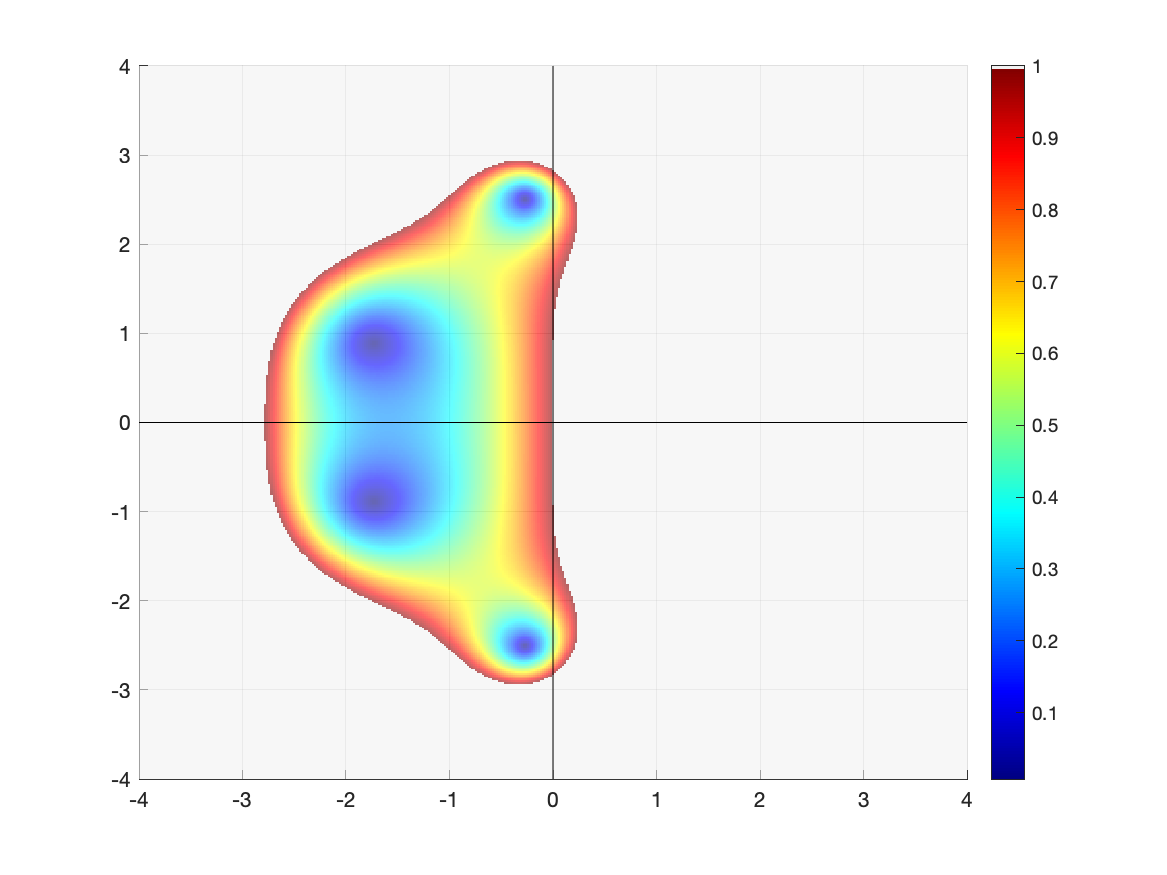
\includegraphics[width=10cm]{graphics/opg1/rk4_stability.png}
    \caption{Stability region of the classical Runge-Kutta method on test equation. The colored region is the stable region.}
    \label{fig1:rk4_stability}
\end{figure}









